
\begin{frame}{Numerical PDE solvers}

{\textbf{PDEs:}} multiphysics, multiscale, constitutive models

{\textbf{Discretisation:}} (grad, curl, div)-conforming, dG, unfitted FEM, hybrid and virtual elements, h/p-adaptivity

{\textbf{(Non)linear solvers:}} multiscale/multilevel solvers strongly coupled to PDE structure (not black-box)

{\textbf{Large scale computations:}} distributed-memory implementations, accelerators, ...

{\textbf{Other ingredients:}} forward/inverse UQ, data-driven parameter identification, ...

\end{frame}

\begin{frame}{Numerical PDE solvers}

E.g., forward UQ on random domains (unfitted, MLMC, multilevel solvers, (inter, intra)-sample parallelism)

\begin{tabular}{cc}
  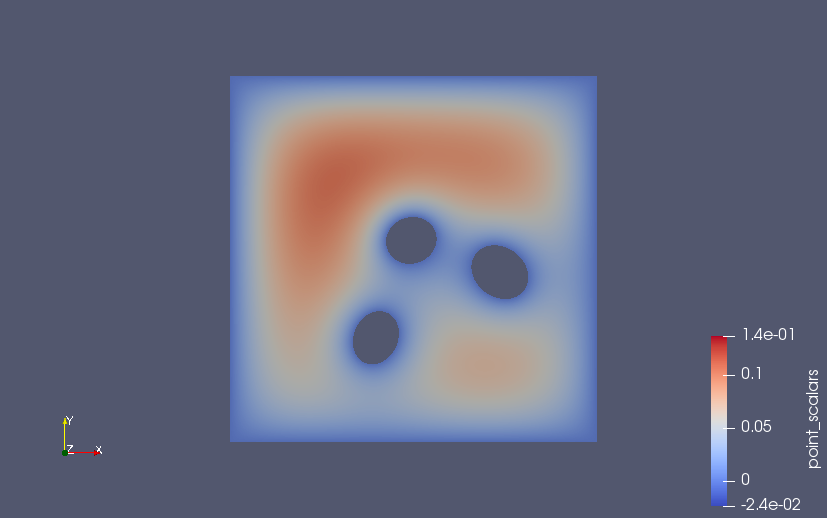
\includegraphics[height=0.23\textwidth]{2dbullets0005.png} &
  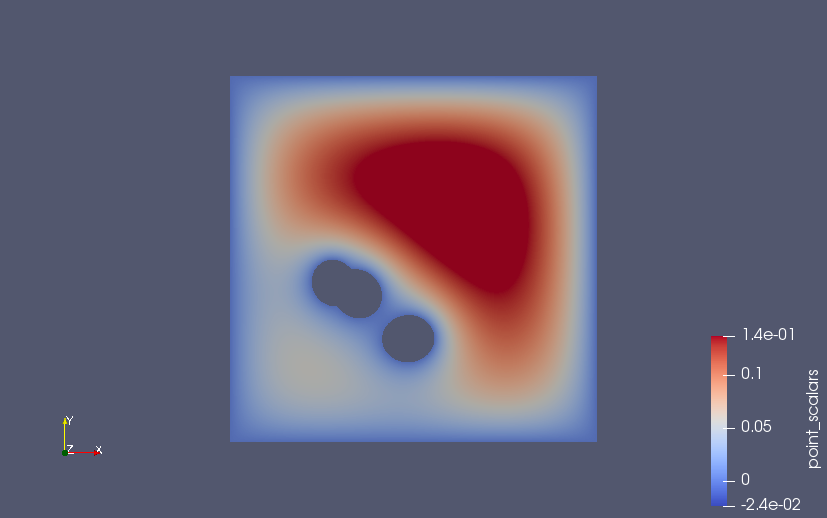
\includegraphics[height=0.23\textwidth]{2dbullets0016.png}  \\
  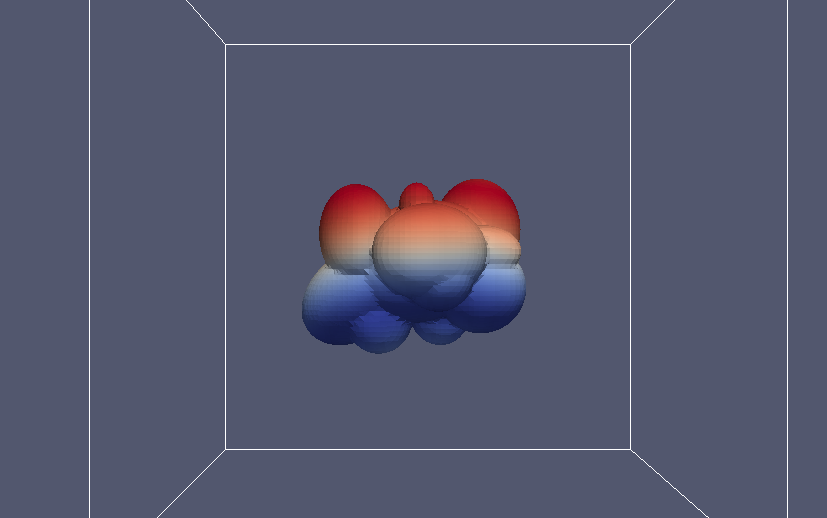
\includegraphics[height=0.23\textwidth]{3dpopcorn0024.png} &
  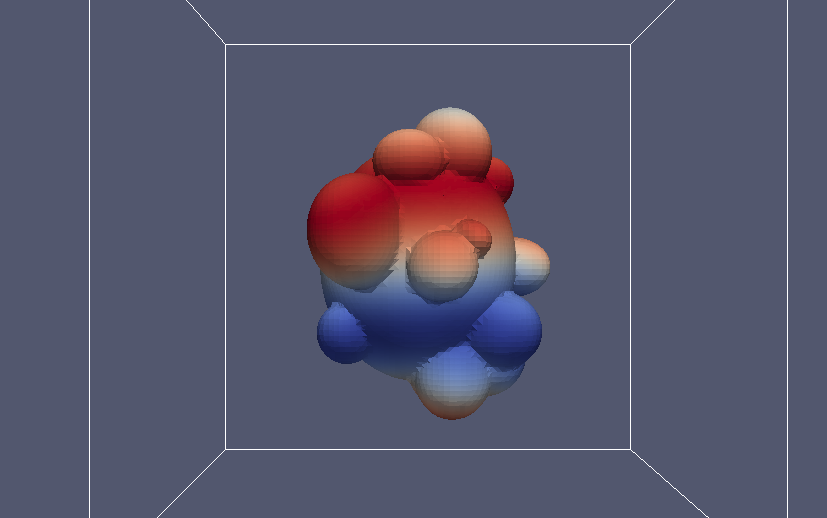
\includegraphics[height=0.23\textwidth]{3dpopcorn0027.png}
\end{tabular}

{\scriptsize

SB, J. Hampton, J. Principe. \emph{Embedded multilevel Monte Carlo for uncertainty quantification in random domains}, arXiv:1911.11965 (2020) }

\end{frame}

\begin{frame}{Computational math labs}

Scientific software + computers are \textbf{our labs}

% We are \textbf{not being paid} for developing high quality scientific software (write papers!)

Advanced algorithms and complex problems require \textbf{advanced software engineering} (extensibility, readability)

Complex problems require \textbf{high-performance} codes (parallel, optimised)

\textbf{Open source} scientific software for reproducible science

\end{frame}

% \begin{frame}Scientific computing labs}
%
% PhD students (3-4y), postdocs (1-3y)
%
% * Starting from scratch every time not an option (hard to reach state-of-the-art interface)
%
% * New algorithms to be implemented, may involve extensions of the library core
%
% * Get into these libraries is *very time-consuming*
%
%
% \end{frame}


\begin{frame}{Scientific computing teams}

Excellent pool of high-performance libraries:

deal.ii, Fenics, FEMPAR, MOOSE, libmesh, Firedrake, DUNE, etc.

\begin{itemize}

  \item  C++ or OO FORTRAN08 (static/compiled languages), some w/ Python interfaces (dynamic language)

  \item Excellent if they provide all you need (\emph{user})

  \item  Far more involved if not (\emph{library developer})

\end{itemize}

\end{frame}

\begin{frame}{Scientific computing teams}

PhD students (3-4y), postdocs (1-3y)

No computer scientists

\begin{block}{Software dev policies}

  \textbf{Reuse:} New algorithms may involve extensions of the PDE library core (\emph{developers}), getting started \emph{very time-consuming} (productivity loss)

  \textbf{Start from scratch:} Academic MATLAB, Python codes (waste previous work, hard to reach state of the art)

\end{block}

\end{frame}

\begin{frame}{Productivity vs performance}

Dilemma: productivity vs performance

\begin{block}{Productivity}
Related to \textbf{dynamic languages} (Python, MATLAB...): More expressive, no compilation step, interactive development (debugging on-the-fly), better for math-related bugs (no benefit from static compilation), no set-up of environment (compilers, system libraries, etc)
\end{block}

\begin{block}{Performance}
Related to \textbf{static languages} (C/C++,FORTRAN,...): Compilers generate highly optimised code
\end{block}

\end{frame}

\begin{frame}{Compromise solutions}

\textbf{Dynamic-static combinations:} vectorised PDE solvers in Python + external pre-compiled libraries (NumPy in C); high-level Python interface of a static PDE library (Fenics, C++), etc.

\begin{itemize}
  \item Constraints over the dynamic code (e.g. vectorisation)
  \item Two-language barrier: When changes require to get into static library
\end{itemize}

\end{frame}

\begin{frame}{Julia lang}

\begin{block}{All-in-one}

\textbf{Productive:} Dynamic language (as Python, MATLAB...)

\textbf{Performant:} Advanced type-inference system + just-in-time (JIT) compilation

\end{block}

21st century FORTRAN, designed for numerical computation (MIT, 2011-)

Solve previous issues: for-loops not a problem, \emph{everything} can be written in Julia (see e.g. Flux for ML, 100$\%$ Julia-code)

% Let us give it a try for PDE discretisation!

\end{frame}

\begin{frame}{Julia features}

\begin{itemize}

  \item \textbf{Not OO:} No inheritance of concrete types (only abstract types), \emph{use composition, not inheritance}, \emph{classify by their actions, not their attributes}...

  \item \textbf{Multiple dispatching paradigm:} functions not bound to types, dispatching wrt all arguments (solving multiple inheritance)

  \item \textbf{Performant Julia code is not obvious:} help JIT compiler to infer types, \emph{type-stability} to allow JIT compiler create performant code

\end{itemize}

\end{frame}

\begin{frame}{Julia universe}

\begin{itemize}

  \item Package manager is awesome

  \item Every project comes with its list of dependencies (automatic process)

  \item Seamless integration with `Github` (register packages, automatically-generated code documentation)

  \item Unit testing and performance tools...

\end{itemize}

\end{frame}

\begin{frame}{Gridap}

Gridap seed started in Christmas 2018... trying to increase productivity in my team

Not good PDE discretisation libraries in Julia

Some key decisions based on previous experience:

\begin{itemize}

  \item Functional-like style i.e. \textbf{immutable objects}, no \emph{state diagram} (just cache arrays for performance)

  \item \textbf{Lazy evaluation} of expressions (implement unary/binary expression trees for types)

\end{itemize}

\end{frame}

\begin{frame}{CellFields}

CellField is a key Gridap type

\begin{block}{CellField}
  Given a cell in a partition $\mathcal{T}$ of a manifold $\mathcal{M}$ (e.g. cells, faces, edges in a mesh), it provides a Field. A Field assings a physical quantity (n-tensor) per space(-time) point in the manifold.

  Given an array of points per cell in $\mathcal{T}$, we can evaluate a CellField, returning an array of scalars/vectors/tensors per cell per point
\end{block}

\end{frame}

\begin{frame}{FEs, Integration, assembly}


We also implement CellField operations:

\begin{itemize}
\item Unary operations: %e.g. $\nabla()$, $\nabla\times()$, $\nabla \cdot()$, etc.
\item Binary operations: inner$(,)$, $\times$, etc.
\end{itemize}

With these types, we represent FE functions, FE bases, constitutive models, etc.

Applying these CellFields to integration points in a numerical quadrature plus operations we can integrate forms and assemble matrices

Let us look at Gridap Tutorial 1
\end{frame}

\begin{frame}{Some comments about the code}

\begin{itemize}

\item Nesting objects into other objects via composition (mesh in FE space in FE function + bilinear form (duck typing) + triangulation + quadrature in FE operator...). All objects are immutable

\item No numerical computations at FEOperator declaration yet, just creating the expression tree ($\nabla()$ and `inner`)

\item Numerically intensive computations deployed in solve

\end{itemize}

\end{frame}

\begin{frame}{Tutorial: nonlinear hyper-elasticity}

Quite complicated PDE

Just some lines of code (laws, residuals, and Jacobians)

\end{frame}

\begin{frame}{Gridap status}

Gridap is pretty comprehensive (big thanks to F Verdugo's amazing work at UPC):

\begin{itemize}
\item Lagrangian, Raviart-Thomas, Nedelec, dG
\item Multifield or multiphysics methods
\item Interaction with GMesh, Pardiso, PETSc...
\item dimension-agnostic (5-dim Laplacian), order-agnostic
\end{itemize}

Quite rich documentation, tutorials, automatic testing, etc.

After 1 year and two developers (not full time!)... highly productive environment

\end{frame}

\begin{frame}{Gridap for teaching}

Objective: same software for research and teaching

\begin{itemize}
\item FE tutorials in \emph{MTH5321 - Methods of computational mathematics}
\item One undergrad AMSI project on \emph{Gridap}: from no idea about FEs/coding to MRI data of velocity of patient-specific aorta to pressure fields in 2 months
\end{itemize}

\end{frame}

\begin{frame}{Gridap future}

This is just the beginning:
\begin{itemize}
  \item Distributed-memory integration/assembly (w/ A Mart\'in)
  \item hp-adaptivity (w/ A Mart\'in)
  \item Historic variables for nonlinear constitutive models
  \item Virtual element methods
  \item Space-time discretisations
  \item Interaction with optimisation, ML, UQ, ODE, automatic diff packages
\end{itemize}
% * Interface w/ BDDC large scale solvers in FEMPAR
\end{frame}

\begin{frame}{Gridap future}

Performance/productivity analysis:
\begin{itemize}
  \item Running FE problems with $O(10^6)$ cells in my laptop in $O(10)$ sec (similar to FEMPAR), \emph{performance analysis} on the way (x2-3 drop in performance OK if x2-3 productivity)
\end{itemize}

\end{frame}

\end{document}

\newcommand{\grad}{\boldsymbol{\nabla}}
\def\u{\boldsymbol{u}}
\def\v{\boldsymbol{v}}
\def\H{\boldsymbol{H}}
\def\b{\boldsymbol{b}}

\begin{frame}{Weak PDE system}
  \begin{block}{Starting point} {Weak form of a PDE} system to simulate in a physical domain $\Omega$
  \end{block}

  \vspace{1cm}



  \begin{columns}
    \begin{column}{0.65\textwidth}

      \begin{overprint}

%        \onslide<1>
%E.g., incompressible Navier-Stokes equations
%        \begin{align*}
%            & \hbox{Find } (\u,p) \in \H^1_0(\Omega) \times L^2_0(\Omega) :  \\
%&  \int_\Omega \v \cdot (\u \cdot \grad) \u
%+ \int_\Omega \nu \grad \v \cdot \grad \u \\
%& - \int_\Omega (\grad \cdot \v) p
%= \int_\Omega \v \cdot \b,  \\
%&  \int_\Omega q \grad \cdot \u = 0, \\
%& \hbox{for any } (\v,q) \in \H^1_0(\Omega) \times L^2_0(\Omega)
%\end{align*}
%
%        \onslide<2>

Abstract PDE system:
$$
u \in X(\Omega) \ : \ a(v,u) = b(v), \quad \forall v \in Y(\Omega),
$$
such that $\| u \|_X \leq \| b \|_{Y'}$ (well-posedness, i.e., bounded by the data)

\vspace{0.1cm}

%{\footnotesize For simplicity: Assume $X(\Omega) = Y(\Omega)$}

      \end{overprint}

    \end{column}
    \begin{column}{0.35\textwidth}

          \includegraphics[height=0.90\textwidth]{nsinc-fig.png}

    \end{column}

  \end{columns}

\end{frame}


%%%%%%%%%%%%%%%%%%%%%%%%%%%%%%%%%%%%%%%%%%%%%%%%%%%%%%%%%%%%%%%%%%%%%%%%%

\begin{frame}{Discrete PDE system}

  \begin{block}{Discretization}

    \begin{itemize}

      \item Replace $X$ by family of $X_\alpha \subset X$ with $\dim(X_\alpha) = C(\alpha) < \infty$

      \item $\alpha$ is a discretization parameter

%      \item $X_\alpha \subset X$ not a requirement...

%     \item ... if perturbed forms $a_\alpha$ and $b_\alpha$ (penalizing $X^\perp \cap X_\alpha$)

    \end{itemize}

  \end{block}

Numerical PDE approximation:
$$
u_\alpha \in X_\alpha(\Omega) \ : \ a(v_\alpha,u_\alpha) = b(v_\alpha), \quad \forall v_\alpha \in Y_\alpha(\Omega)
$$

\begin{itemize}
  \item \underline{Stability:} $\| u_\alpha \|_{X} \leq \| b \|_{Y'}$% where $X(\alpha) \doteq X + X_\alpha$
  \item \underline{Convergence:} $\| u - u_\alpha \|_{X} \leq E(u,\alpha)$ s.t. $E(u,\alpha) \to 0$ as $\alpha \to 0$
\end{itemize}

%  \begin{block}{Approximability}
%  Define a sequence of spaces $\{ X_\alpha \}$ such that
%  $$\sup_{v \in X} \inf_{v_\alpha \in X_\alpha} \| v - v_\alpha \|_X \to 0 \quad \hbox{ as  } \quad \alpha \to \infty$$
%  \end{block}
%
\end{frame}


\def\mesh{\mathcal{T}}
\begin{frame}{Discrete spaces}


  \begin{overprint}

%    \onslide<1>
%
%    Spectral methods: polynomials up to order $\alpha$ in $\Omega$
%
%    \vspace{0.4cm}
%
%    \begin{tabular}{cccc}
%      \includegraphics[height=0.15\textwidth]{shfs_0.png} &
%      \includegraphics[height=0.15\textwidth]{shfs_1.png} &
%      \includegraphics[height=0.15\textwidth]{shfs_2.png} &
%      \includegraphics[height=0.15\textwidth]{shfs_3.png} \\
%      $\alpha = 0$ &
%      $\alpha = 1$ &
%      $\alpha = 2$ &
%      $\alpha = 3$
%    \end{tabular}
%
%    Only useful for \emph{very smooth} problems, otherwise no approximability
%
%    \onslide<2>
%
    Finite elements (volumes) when $\Omega$ non-trivial: \\
    {\footnotesize (otherwise also finite differences, spectral (if high smoothness), etc)}

    \vspace{0.2cm}

    \begin{tabular}{cccc}
      \includegraphics[trim=10cm 1cm 10cm 1cm,clip,height=0.15\textwidth]{mesh1.pdf} &
      \includegraphics[trim=10cm 1cm 10cm 1cm,clip,height=0.15\textwidth]{mesh2.pdf} &
      \includegraphics[trim=10cm 1cm 10cm 1cm,clip,height=0.15\textwidth]{mesh4.pdf} &
      \includegraphics[trim=10cm 1cm 10cm 1cm,clip,height=0.15\textwidth]{mesh8.pdf} \\
      $\mesh_{\alpha=0}$ &
      $\mesh_{\alpha=1}$ &
      $\mesh_{\alpha=2}$ &
      $\mesh_{\alpha=3}$
    \end{tabular}

    \begin{itemize}

      \item Consider a partition $\mesh_0$ of $\Omega$ + uniform refinement

      \item Cell-wise polynomial spaces + inter-cell trace continuity

%      \item Approximability even with low regularity

    \end{itemize}
  %    \includegraphics[width=0.5\textwidth]{fe2.png}

  \begin{block}{Linear approximation}
    Such approximation is linear, i.e.,
    $$
    u_\alpha \in X_\alpha = {\rm span}\{ \phi_1, \phi_2, \ldots, \phi_{\#} \},
  \quad \# \hbox{ number of DOFs}
    $$
    %and $X_\alpha$ does not depend on the exact solution $u$
      Convergence (algebraic rate)
        $
        \| u - u_\alpha \|_{X} \lesssim \#^{\frac{\beta}{D}}
        $
         for $\beta > 0$ that depends on polynomial order, regularity of $u$, etc.
  \end{block}

  \end{overprint}

%$\alpha$ can be understood as uniform levels of refinement

%Issue: How to generate $\mesh$; geometrical error

\end{frame}


\def\dofs{\boldsymbol{\xi}}
\def\A{\boldsymbol{\mathcal{A}}}
\def\J{\boldsymbol{\mathcal{J}}}



\begin{frame}{Adaptive FEM}

  \begin{block}{Nonlinear approximation: Adaptive FEM}

      \emph{A posteriori error estimates:} cell-wise quantities $\{\eta_K\}_{K \in \mesh_\alpha}$
    $$
    \sum_{K \in \mathcal{T}_\alpha} \eta_K(u_\alpha) \lesssim \| u - u_\alpha \|_{X} \lesssim \sum_{K \in \mathcal{T}_\alpha} \eta_K(u_\alpha),
    $$

    \begin{itemize}
  \item Adaptive refinement, $\mesh_\alpha = \mesh_\alpha(u)$ for $\alpha > 0$

  \item Exponential convergence, i.e., $\| u - u_\alpha \| \lesssim e^{\#^\gamma}$

%  \item Deep neural networks are another kind of nonlinear approximation
  \end{itemize}
\end{block}


    \begin{tabular}{cccc}
      \includegraphics[trim=55cm 10cm 6cm 1cm,clip,height=0.25\textwidth]{circular-discontinuity-1ref.png}&
      \includegraphics[trim=55cm 10cm 6cm 1cm,clip,height=0.25\textwidth]{circular-discontinuity-2ref.png}&
      \includegraphics[trim=55cm 10cm 6cm 1cm,clip,height=0.25\textwidth]{circular-discontinuity-3ref.png}&
      \includegraphics[trim=55cm 10cm 6cm 1cm,clip,height=0.25\textwidth]{circular-discontinuity-8ref.png}\\
      $\mesh_{\alpha=1}$ &
      $\mesh_{\alpha=2}$ &
      $\mesh_{\alpha=3}$ &
      $\mesh_{\alpha=8}$
    \end{tabular}


\end{frame}


\begin{frame}{Linearization}
  Nonlinear discrete problem wrt DOF values $\dofs = [ \xi_1, \cdots, \xi_n ]^T$,
  $$\A(\boldsymbol{\xi}) = \boldsymbol{b}, \qquad u = \sum \phi_i \xi_i $$

  \begin{columns}

    \begin{column}{0.5\textwidth}

      After linearization, e.g., using Newton's method
      $$\J \dofs \doteq \frac{{\rm d}\A}{{\rm d}\dofs}(\dofs^*) \delta\dofs
      \boldsymbol{b} - \A(\dofs^*) = \boldsymbol{r}(\dofs)$$

      Linear and sparse system of equations

    \end{column}

    \begin{column}{0.4\textwidth}
      \begin{tabular}{c}
        \frame{\includegraphics[width=0.85\textwidth]{matrix2.png}} \\
      $\J$
    \end{tabular}

    \end{column}
  \end{columns}

      \begin{block}{Scalable linear PDE solvers}
        Define preconditioner $\widetilde \J$ \emph{spectrally equivalent} to $\J$, i.e., $\| \widetilde \J^{-1} \J \| \| \J^{-1} \widetilde \J \| \simeq 1$
        s.t. $\tilde \J^{-1} \boldsymbol{r}$ is \emph{highly parallel}, i.e.,
      $$
      {\rm time}(\widetilde \J^{-1}\boldsymbol{r}) \approx
      {\rm time}(\J_1^{-1}\boldsymbol{r})
      + {\rm time}(\J_2^{-1}\boldsymbol{r})
      + \ldots
      + {\rm time}(\J_P^{-1}\boldsymbol{r})
      $$
            Scalable preconditioning (not covered Today) can efficiently run on largest supercomputers today
      \end{block}

\end{frame}

%\begin{frame}{Computer resources}
%
%
%  \begin{columns}
%
%    \column{0.5\textwidth}
%
%  Numerical PDEs are computationally very intensive (3D+1D)
%
%  \vspace{0.1cm}
%  \begin{tabular}{c}
%            \includegraphics[width=0.6\textwidth]{climate.jpg} \\
%          {\scriptsize Climate modelling (ACME project, DOE)} \\
%          \includegraphics[width=0.6\textwidth]{direct-numerical-simulation.png} \\
%          {\scriptsize Combustion modelling (EXACT project, DOE)}
%        \end{tabular}
%
%    \column{0.5\textwidth}
%
%  Supercomputers are distributed-memory machines
%
%  \includegraphics[width=0.6\textwidth]{cluster.png}
%
%  \includegraphics[width=0.8\textwidth]{parallelcomp.png}
%
%  Hardware-aware numerical algorithms
%
%  \end{columns}
%
%  \begin{block}{Scalable numerical methods}
%    An algorithm that can be re-stated as $P$ indepedendent tasks + a negligible inter-task communications
%  \end{block}
%
%
%\end{frame}
%
%\begin{frame}{Parallel computing}
%
%  \begin{columns}
%    \begin{column}{0.5\textwidth}
%
%      \begin{block}{1. Mesh generation}
%%        Compute partition $\mathcal{T}_0$ of $\widetilde \Omega \approx \Omega$
%      Delaunay triangulation (hard to parallelize) to compute partition $\mathcal{T}_0$, an approximation of $\Omega$
%      \end{block}
%
%      \begin{center}
%        \begin{figure}
%          \includegraphics[width=0.6\textwidth]{mesh.png}
%        \end{figure}
%      \end{center}
%      \vspace{-0.1cm}
%
%      \begin{block}{3. Numerical integration}
%           Embarrassingly parallel
%           $$ \hbox{e.g.,} \quad [\J_i]_{ab} = \int_{K \in \mesh_0^i} \grad \phi_a \cdot \grad \phi_b  \quad $$
%            for ${i=1,\ldots,P}$
%      \end{block}
%    \end{column}
%    \begin{column}{0.6\textwidth}
%
%      \begin{block}{2. Mesh partition}
%      %  Partition of $\mesh_0$ into sub-meshes $\mesh_0^1, \mesh_0^2, \ldots, \mesh_0^P$
%         Graph partitioning (inherently sequential, poor parallelism)
%      \end{block}
%
%      \includegraphics[width=0.8\textwidth]{partition.png}
%
%      \begin{block}{4. Scalable solvers}
%           %{\bf Scalable} algorithms are very complex % (e.g., multilevel domain decomposition, multigrid)
%            Whereas matvec is parallel, $$\J \dofs = {\rm assemble}(\J_1 \dofs_1, \cdots, \J_n \dofs_n),$$ $\J^{-1} \boldsymbol{r}$ is a tightly coupled global problem
%
%            Scalable preconditioning (not covered Today) in good shape
%            %    \item {\color{red} {\bf First part of the talk}}
%      \end{block}
%
%     % \begin{center}
%     %   \begin{figure}
%          %\includegraphics[width=0.4\textwidth]{photos/weak-scaling-image.png}
%          %\includegraphics[width=0.4\textwidth]{photos/weak-scaling-bone.png}
%     %   \end{figure}
%     % \end{center}
%
%    \end{column}
%  \end{columns}
%\end{frame}
%
%\begin{frame}{Preconditioning}
%
%Linear systems are global and efficient parallelization far from obvious
%
%%Only very complex algorithms attain the objective
%
%\begin{block}{Preconditioning}
%  Design $\tilde \J$ such that
%  \begin{enumerate}
%    \item $\tilde \J$ \emph{spectrally equivalent} to $\J$, i.e., $\| \widetilde \J^{-1} \J \| \| \J^{-1} \widetilde \J \| \simeq 1$
%      %$\kappa(\tilde \J^{-1}\J) \simeq 1$
%
%    \item  $\tilde \J^{-1} \boldsymbol{r}$ is \emph{highly parallel}, i.e.,
%      $$
%      {\rm time}(\widetilde \J^{-1}\boldsymbol{r}) \approx
%      {\rm time}(\J_1^{-1}\boldsymbol{r})
%      + {\rm time}(\J_2^{-1}\boldsymbol{r})
%      + \ldots
%      + {\rm time}(\J_P^{-1}\boldsymbol{r})
%      $$
%
%    \item \emph{Optimal} cost, i.e., ${\rm flops}(\widetilde \J^{-1} \boldsymbol{r}) \simeq {\rm flops}(\J \boldsymbol{b})$
%  \end{enumerate}
%\end{block}
%
%Iterative Krylov method over $\widetilde \J^{-1} \J \dofs = \widetilde \J^{-1} \boldsymbol{r}$ (CG, GMRES...)
%
%
%\end{frame}
%
%
%
% \begin{frame}{Scalable PDE linear solvers}
%% Scalable PDE solvers are complex (to analyze and implement)
%
% \begin{block}{Multilevel domain decomposition}
%   \begin{itemize}
%     \item Idea: Define space with {\bfseries relaxed inter-proc continuity} (recursively)
%   \item {Local subdomain problems} at all levels (L1, L2, ...) + weak communications
% \end{itemize}
% \end{block}
%% \item \albf{1}{Multilevel DD} preconditioner, e.g., MLBDDC\footnote{J. Mandel, B. Sousedik, C. Dohrmann. Multispace and multilevel BDDC. \emph{Computing}, pp. 55--85 (2008)} based on a {hierarchy of meshes/functional spaces}
%
%% \begin{overprint}
%
%%   \onslide<1>
% \begin{tabular}{ccc}
%   \includegraphics[width=0.3\textwidth]{backward_facing_step_3D_mesh.pdf}&
%   \includegraphics[width=0.3\textwidth]{backward_facing_step_3D_128parts.pdf}&
%   \includegraphics[width=0.3\textwidth]{backward_facing_step_3D_8parts.pdf}\\
%   $X_\alpha^{(0)} \quad \subsetneq$ & $X_\alpha^{(1)} \quad \subsetneq$ & $X_\alpha^{(2)} \ldots$
% \end{tabular}
%% {\footnotesize FE mesh \hspace{1.5cm} Subdomains (L1)  \hspace{1.5cm}  Subdomains (L2)  }
%
% \vspace{0.5cm}
% Well-developed math theory, $\kappa(\widetilde \J^{-1} \J) \simeq 1$ for many systems of PDEs (Thermal, elasticity, Maxwell, Darcy, Stokes, multiphysics couplings; highly heterogeneous problems, etc)
%
%
% Scalable implementation up to $>2$ million proc's and $10^{11}$ (and beyond)
%
%% \onslide<2>
%%
%%  \vspace{0.5cm}
%%   Excellent results at large scales
%%\begin{center}
%%\vspace{-1ex}
%%\begin{tabular}{c@{}c}
%%\includegraphics[width=0.5\textwidth]{weak_3D_H_div_h_4_3_bddc_ce_iter}  &
%%\includegraphics[width=0.5\textwidth]{weak_3D_H_div_h_4_3_bddc_ce_tot} \\
%%\end{tabular}
%%\end{center}
%% \end{overprint}
%
%
%
% \end{frame}
%

 \begin{frame}{Geometry discretization}

   \begin{columns}
     \begin{column}{0.5\textwidth}
       \begin{block}{Trivial domains} Octree meshes w/ adaptive mesh refinement
   \begin{itemize}

     \item Scalable generation and partition (space-filling curves)

     \item Automatic process (no human intervention)

    \end{itemize}
  \end{block}



     \end{column}
     \begin{column}{0.5\textwidth}
\begin{figure}
\includegraphics[width=0.75\textwidth]{amr3.jpeg}
\includegraphics[width=0.3\textwidth]{fig_filling_curve_a.pdf}
\includegraphics[width=0.3\textwidth]{fig_filling_curve_b.pdf}
\end{figure}

     \end{column}
   \end{columns}

   \begin{columns}
     \begin{column}{0.5\textwidth}

       \begin{block}{Complex domains}
         Unstructured meshes
       \begin{itemize}

         \item Not scalable generation/partition

         \item {\bfseries Not automatic}  (human intervention)

         \item About $80\%$ of the time in CAE

         \item Interfaces, stochastic domains (?)

%         \item Adaptive FEM complicated ($)

       \end{itemize}
     \end{block}

     \end{column}
     \begin{column}{0.4\textwidth}

       \vspace{1cm}
       \begin{tabular}{c}
       \includegraphics[width=1.0\textwidth]{complexmesh.png} \\
%       $\mathcal{T}_0$ partition of $\Omega$ (approx.)
     \end{tabular}

     \end{column}
   \end{columns}



 \end{frame}



\begin{frame}
\frametitle{ Embedded FEM }


\begin{columns}[onlytextwidth,t]

\column{0.33\textwidth}

\centering

\includegraphics[width=0.9\textwidth]{fig_intro_imb_1.png}

\column{0.33\textwidth}

\centering

\includegraphics[width=0.9\textwidth]{fig_intro_imb_3.png}


\column{0.33\textwidth}

\centering

\includegraphics[width=0.9\textwidth]{fig_intro_imb_2.png}


\vspace{1em}


\end{columns}

\begin{overprint}
\onslide<1>
\begin{block}{Cut cell integration (two techniques)}
  \vspace{0.2cm}
\begin{itemize}
  \item \emph{Implicitization of surfaces}  ($\boldsymbol{\chi}_\alpha \in X_\alpha$ s.t. $\Omega \approx \{ \boldsymbol{x} : \boldsymbol{\chi}_\alpha(\boldsymbol{x}) = 0 \}$)
    %` w`such that $\+ marching tetrahedra (computer vision)
  \item Surface mesh generation $\partial \Omega_\alpha$ + exact integration on $\Omega_\alpha$
\end{itemize}



  %\begin{align*}
  %  \int_{\Omega\cap K} \nabla \varphi_i \cdot \nabla \varphi_j &+ \int_{\partial\Omega\cap K} \beta \varphi_i  \varphi_j + \cdots \\[1em]
  %                      & =\sum_{\mathrm{tet}}\int_{\mathrm{tet}} \nabla \varphi_i \cdot \nabla \varphi_j + \sum_{\mathrm{tri}}\int_{\mathrm{tri}} \beta \varphi_i \varphi_j + \cdots
  %\end{align*}
\end{block}

%  \vspace*{1em}

  \begin{center}
 \includegraphics[width=0.3\textwidth]{fig_cut_int_1a.pdf}\hspace*{2em}
% \includegraphics[width=0.3\textwidth][trim=1cm 1cm 1cm 1cm,clip]{bunny.jpg}
  \hspace*{2em}
  \includegraphics[trim=13.3cm 0cm 0cm 14.2cm,clip,height=0.20\textwidth]{bunny.jpg}
\end{center}


%  \includegraphics[width=0.3\textwidth]{fig_cut_int_2a.pdf}
%  \begin{tabular}{cc}
%    \includegraphics[width=0.2\textwidth]{broccoli.jpg} & \emph{\footnotesize Exact geometry is a chimera}
%\end{tabular}

\onslide<2>

  \begin{columns}[onlytextwidth]

    \column{0.6\textwidth}


    \begin{block}{Ill-conditioning}

      \begin{itemize}
        \item[1)] Standard FEM on body-fitted meshes
          \begin{equation*}
            \kappa(\J) \simeq  \min_{K \in \mesh_\alpha} {\rm diam}(K)^{-2}
          \end{equation*}
        \item[2)] Standard FEM on cut meshes
          \begin{equation*}
            \kappa(\J) \simeq  \min_{K \in \mesh_\alpha} |\eta_K|^{-(2p+1-2/D)}
          \end{equation*}
      \end{itemize}



      %* Estimates for the Poisson eq.\par
      %{\small [de Prenter et al. 2017, C. Johnson (book)]}

    \end{block}

    \column{0.36\textwidth}

    \centering
    \includegraphics[width=0.9\textwidth]{betas_d.pdf}

  \end{columns}

\end{overprint}


\end{frame}


\begin{frame}{Aggregated FEM}
  \begin{columns}[onlytextwidth]

    \column{0.5\textwidth}

    \underline{Ingredient 1:} Cell aggregation algorithm s.t.
 $\max_{K \in \mesh_\alpha} {\eta_K} \gtrsim 1$

 \vspace{0.5cm}

 \begin{tabular}{c}
    \includegraphics[width=0.5\textwidth]{fig_dof_to_cell_map_12.pdf} \\
    {\footnotesize Aggregated mesh}
    \end{tabular}

    \vspace{0.2cm}
    \underline{Ingredient 2:} FE spaces on aggregated meshes
    \begin{itemize}
      \item Aggregate-wise polynomial space
      \item Enforce trace continuity
    \end{itemize}

    \column{0.5\textwidth}



    \begin{block}{Numerical analysis}
      Condition number as body-fitted methods
      $$\kappa(\J) \simeq  \min_{K \in \mesh_\alpha} {\rm diam}(K)^{-2}$$

      Idem for convergence estimates
    $$
    \| u - u_h \|_{X} \lesssim \max_{K \in \mesh_\alpha} {\rm diam}(K)^{p}$$

    and stability for coercive and indefinite problems (Stokes)%, inverse/trace inequalities...
        \end{block}

  \end{columns}
\end{frame}

\begin{frame}{Current and future work}
%
  \vspace{-0.5cm}
  \underline{Current state}: {\bfseries Automatic}, scalable, robust, adaptive FEs on octree meshes for complex geometries

  \begin{tabular}{cccc}
    \includegraphics[width=0.50\textwidth]{CBA-mesh-volume-2.png} &
    \includegraphics[width=0.50\textwidth]{Spiral-mesh-volume-2.png}
%    \includegraphics[width=0.53\textwidth]{spiral.png} &
%    \includegraphics[width=0.53\textwidth]{spiral_mesh_4.png}
  \end{tabular}


%  \vspace{1cm}

  \begin{columns}

    \column{0.3\textwidth}

    \includegraphics[width=0.8\textwidth]{broccoli.jpg}

    \emph{\footnotesize Exact geometry is a chimera}


    \column{0.75\textwidth}
    \begin{block}{Recent/future work}
  \begin{itemize}

    \item Multilevel Monte Carlo methods on random domains

    \item Quantify {\bfseries geometrical error} $|\Omega - \Omega_\alpha|$ and effect on a priori $\| u - u_\alpha \|_{X}$ and a posteriori $\eta_K$ error estimates

    \item \emph{Space-time} formulations, i.e., $\Omega \times (0,T]$

    \item \emph{Interface} problems where $\Omega$ is an unknown

  \end{itemize}
\end{block}

\end{columns}

\end{frame}


%\begin{frame}{Further topics}
%
%Multilevel Monte Carlo for PDEs on uncertain domains
%
%Variance-reduction methods based on hierarchical meshes
%
%Stochastic domains
%
%Growing geometries in 3D printing thermal simulations
%
%Topology optimization
%
%Geometry grows in time, BFM not possible
%
%\end{frame}

\end{document}
